
RNA molecules play diverse roles in encoding and regulating genetic information, and much of this versatility can be traced to the formation of intricate RNA structures. To this end, chemical probing methodologies provide a general and rapid means to mapping RNA secondary and tertiary structure at single-nucleotide resolution~\citep{weeks2010}.

There exist many chemical probing techniques, most of which have common experimental procedures, as follows. Given an RNA of interest folded in solution, a chemical reagent modifies the RNA, either cleaving it or forming a covalent adduct with it at a rate correlated with the extent of structure at each nucleotide. Examples of such chemical reagents include hydroxyl radicals, 2$'$-OH acylating chemicals (SHAPE), dimethyl sulfate (DMS), and CMCT~\citep{Weeks2010295}. Subsequent reverse transcription detects the modification sites as stops to primer extension at nucleotide resolution. The resulting complementary DNA (cDNA) fragments are resolved in sequencing gels followed by individually quantifying band intensities. Prior to the mid-2000s, the bottlenecks were the final steps (gel running and band quantification).

To resolve fragments in a more high-throughput fashion, capillary electrophoresis (CE) was developed and is reaching wide use. CE-based chemical probing can easily produce tens of thousands of individual electrophoretic bands from a single experiment, leading to recent breakthroughs in two-dimensional mapping of complex RNA structures ~\citep{kladwangmutatemap2011} and their excited states \citep{tian2014nature}, and extension to large complexes such as ribosomes~\citep{weeksbiochemistry} and viruses~\citep{weeksplos2009,weeksnature2009} and to RNA design problems~\citep{daskaranicolasbaker2010,lee2014pnas}. Further developments in next-generation sequencing readouts are promising but still show biases compared to CE measurements \citep{Lucks2011,Kladwang2014}.

Analyzing a large number of electrophoretic traces from a high-throughput structure-mapping experiment is time-consuming and poses a significant informatic challenge, requiring a set of robust signal-processing algorithms for accurate quantification of the bands embedded in these traces. Software methods for CE analysis include capillary automated footprinting analysis (CAFA; \citealp{mitra2008high}), ShapeFinder~\citep{vasa2008shapefinder}, high-throughput robust analysis for capillary electrophoresis (HiTRACE; \citealp{Yoon2011}), fast analysis of SHAPE traces (FAST; \citealp{Pang2011}), and QuShape~\citep{Karabiber2013}.

A typical high-throughput CE analysis pipeline consists of the following steps~\citep{Yoon2011,Karabiber2013,Kladwang2014}: preprocessing such as normalization and baseline adjustment, alignment, peak detection, band annotation, and peak fitting. Among these, band annotation refers to the process of mapping each band in an electrophoretic trace to a position in the nucleic acid sequence. For verification, visual inspection in this phase is inevitable to some extent. However, in practice, this band annotation step often takes significant human efforts in CAFA and SHAPEfinder, for they were designed to focus more on alignment and peak fitting. HiTRACE, QuShape, and FAST have provided improved levels of band annotation support, but band annotation remains still the most time-consuming steps of these pipelines for large data sets that probe an RNA under many different conditions or with many mutations.

This paper describes a dynamic-programming based approach to automated band annotation for such large CE data sets. These data sets frequently involve multiple aligned traces for each RNA, based on sequencing ladders for the four different nucleotide types, different chemical modifiers SHAPE, and/or chemical modification under different solution conditions or with different mutations. The central innovation herein is an accurate and well-tested procedure to combine information across these multiple traces to create a single consensus band annotation with accuracy approaching that of manual annotation. Figure~\ref{f:overview} shows the overview of the proposed methodology.


%%%%%%%%%%%%%%%%%%%%%%%%%%%%%%%%%%%%%%%%%%%%%%%%%%%%%%%%%%%%%%%%%%%%%%%%%%%%%%%%
% OVERVIEW
%%%%%%%%%%%%%%%%%%%%%%%%%%%%%%%%%%%%%%%%%%%%%%%%%%%%%%%%%%%%%%%%%%%%%%%%%%%%%%%%
\begin{figure}
\centering
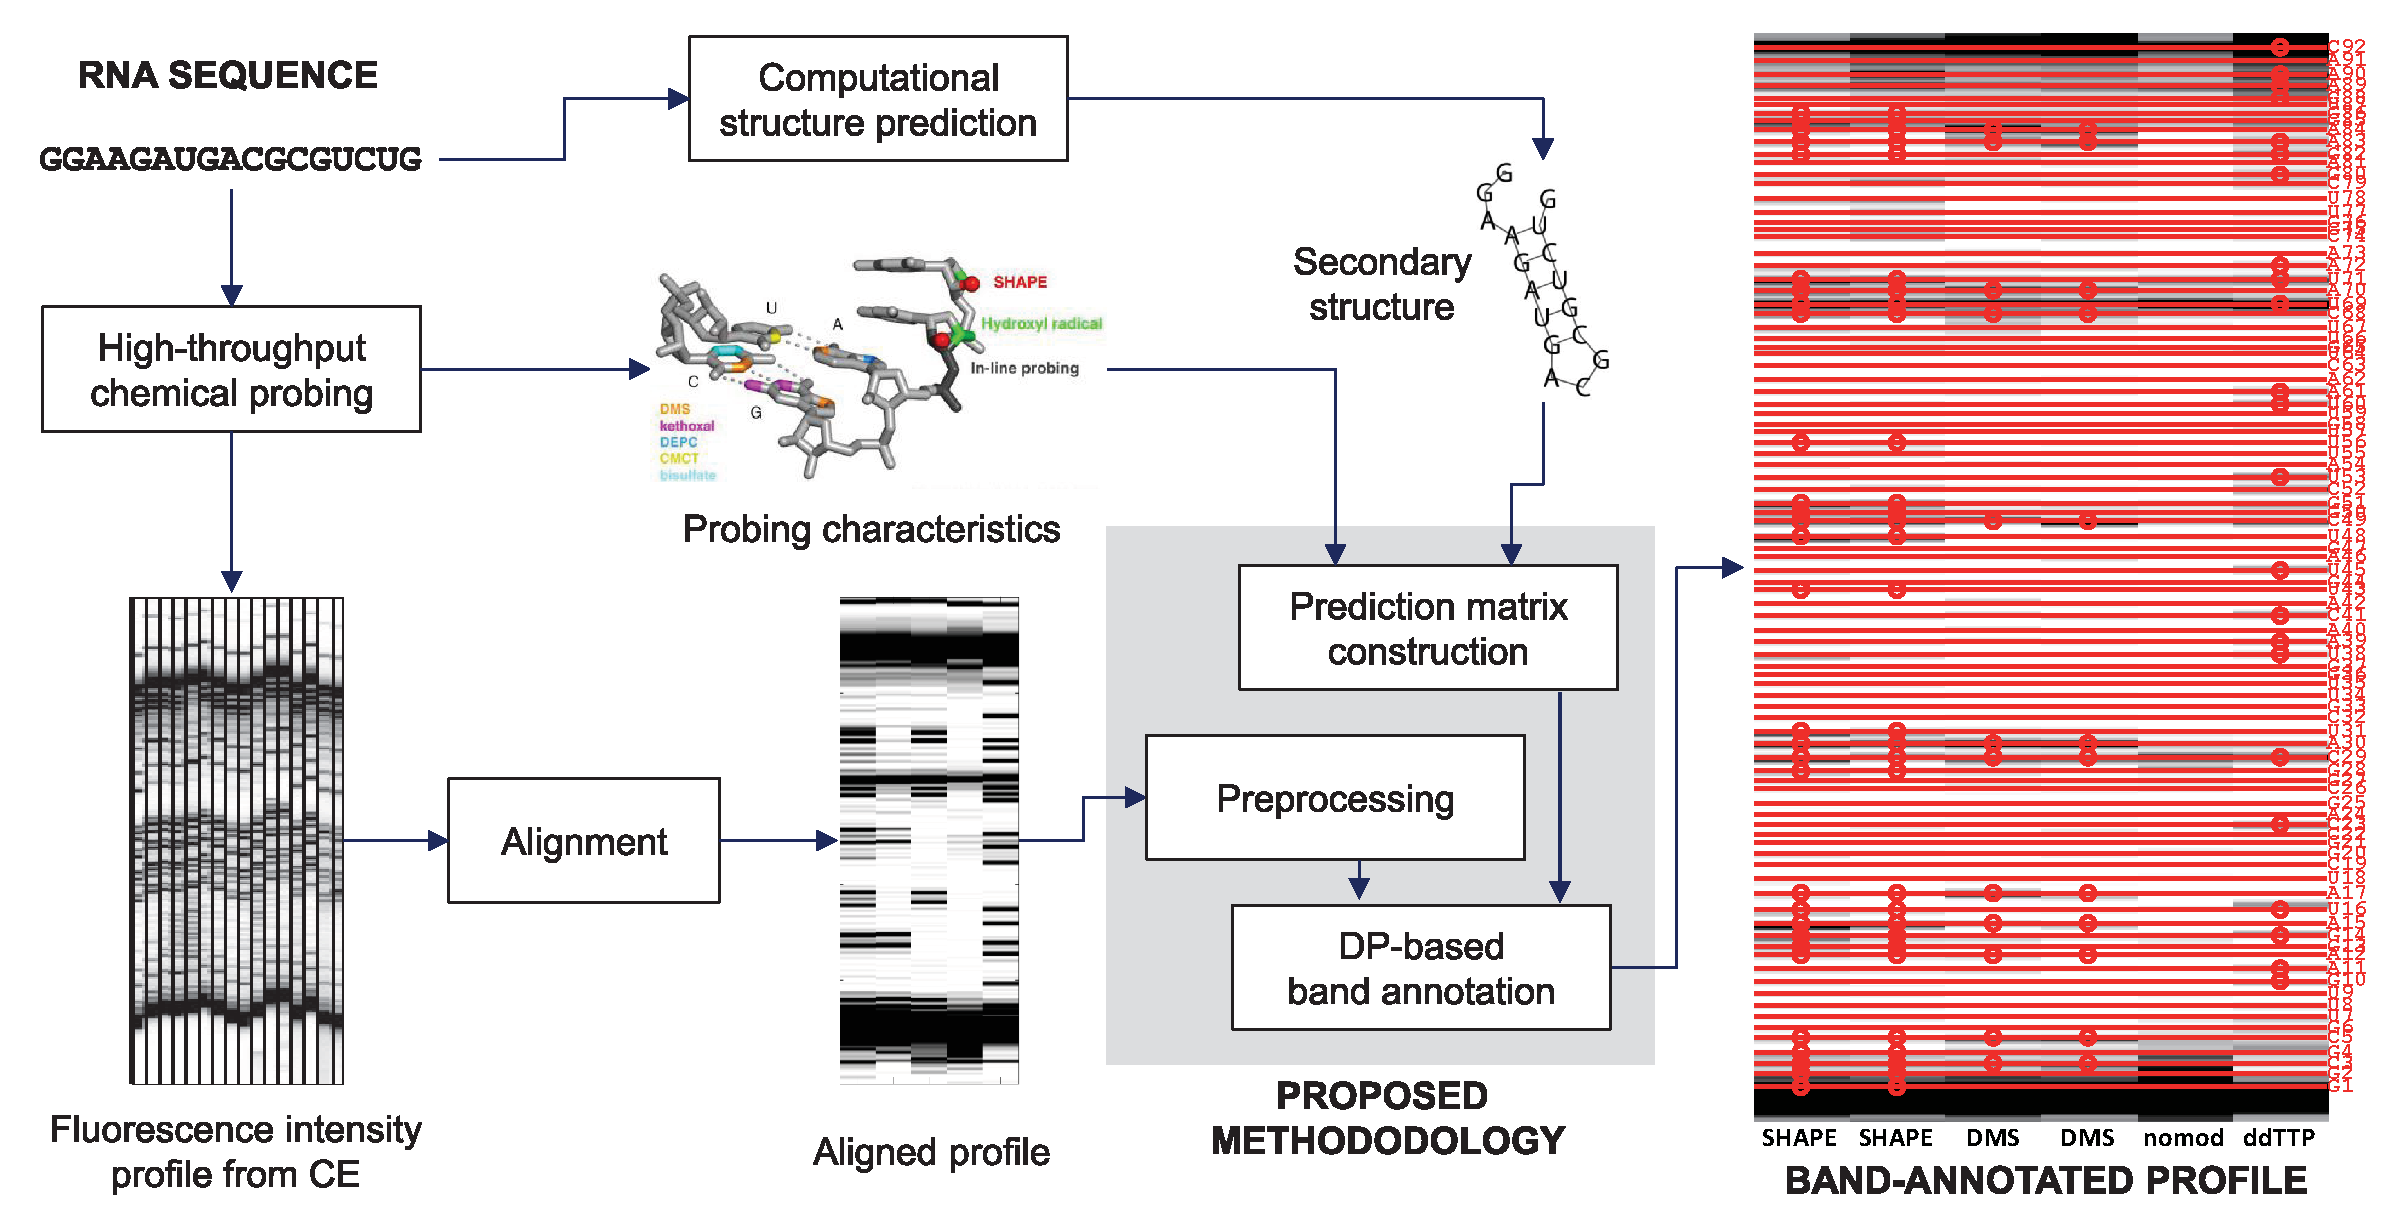
\includegraphics[width=\linewidth]{figures/intro_overview2}
\caption{Overview of the proposed dynamic-programming-based band annotation methodology. Given an RNA sequence, we carry out high-throughput structure-mapping experiments, producing a number of capillary electrophoresis (CE) traces. If available or estimated through computational prediction, we also provide the RNA's secondary structure. From this information and the characteristics of the chemical probing method used, we derive a prediction matrix that stores expected interaction patterns across the residues and traces. Based on the aligned CE traces and prediction matrix, we apply a dynamic-programming approach that finds the optimal selection of the band locations under a well-defined scoring scheme.}
\label{f:overview}
\end{figure}
%%%%%%%%%%%%%%%%%%%%%%%%%%%%%%%%%%%%%%%%%%%%%%%%%%%%%%%%%%%%%%%%%%%%%%%%%%%%%%%%


